% !TEX root = ../patchEmbeddings_review.tex

\section{Related work} \label{sec:related_work}
\textbf{Proposal-based methods} -- Many of the recent successful instance segmentation methods on natural images are \emph{proposal based}: they first perform object detection, for example by predicting anchor boxes \cite{ren2015faster}, and then assign a class and a binary segmentation mask to each detected bounding box, either convolutionally \cite{he2017mask,porzi2019seamless,liu2018path,yang2012layered,li2017fully,ladicky2010and,hariharan2014simultaneous,chen2015multi,dai2016instance,liang2016reversible} or in a recurrent fashion by sequentially generating instances one-by-one \cite{romera2016recurrent,ren2017end}. 
% However, in this work we focus on 3D neuron segmentation for connectomics, which is a field of neuroscience where instances/neurons cannot be approximated by bounding boxes. \TODO{Remove?}

\textbf{Proposal-free methods} on the other hand directly group pixels into instances. 
% whereas the template matching \cite{uhrig2016pixel} deploys scene depth information.
Recent approaches use metric learning to predict high-dimensional associative pixel embeddings that map pixels of the same instance close to each other, while mapping pixels belonging to different instances further apart, e.g. \cite{kong2018recurrentPix,fathi2017semantic,newell2017associative,de2017semantic} on natural images and \cite{lee2019learning} for neuron segmentation in connectomics. % kulikov2018instance
Final instances are then retrieved by applying a clustering algorithm and a post-processing step is needed to merge instances that are larger then the field of view of the network. 
Other proposal-free methods predict the relative coordinates of the instance center \cite{neven2019instance,cheng2019panopticdeeplab}, whereas others generate the mask of the instance associated to a given seed point \cite{sofiiuk2019adaptis} or  
learn a watershed transform by predicting its gradient direction \cite{bai2017deep}. 

\textbf{Aggregating \maskname masks} -- 
The line of research closest to our predicts densely located \maskname masks in a sliding window style across the entire image. The work of \cite{liu2016multi} aggregates overlapping masks and compute intersection over union scores between them.
In neuron segmentation, flood-filling networks \cite{januszewski2018high} and MaskExtend \cite{meirovitch2016multi} use a CNN to iteratively grow one instance/neuron at the time, merging one mask after the other. Recently, the work of \cite{meirovitch2019cross} made the process more efficient by employing a combinatorial encoding of the segmentation, but the method remains orders of magnitude slower as compared to the convolutional one proposed here, since in our case all masks are predicted at the same time and for all instances.
The most closely related to ours is the unpublished independent work from \cite{hirsch2020patchperpix}, where a very similar model is applied to the BBBC010 benchmark microscopy dataset of \emph{C. elegans} worms. However, here we propose a more efficient model that scales to 3D data and provide an extensive comparison to related models predicting long-range pixel-pair affinities. 
%  a parameter-free algorithm to aggregate overlapping masks.
% \TODO{Fred?}

\begin{figure}[t]
\centering
        % \includegraphics[width=0.4\textwidth,trim=0.25in 0.25in 0.68in 0.36in,clip]{./figs/SSBM_experiments.pdf} % 0.45
        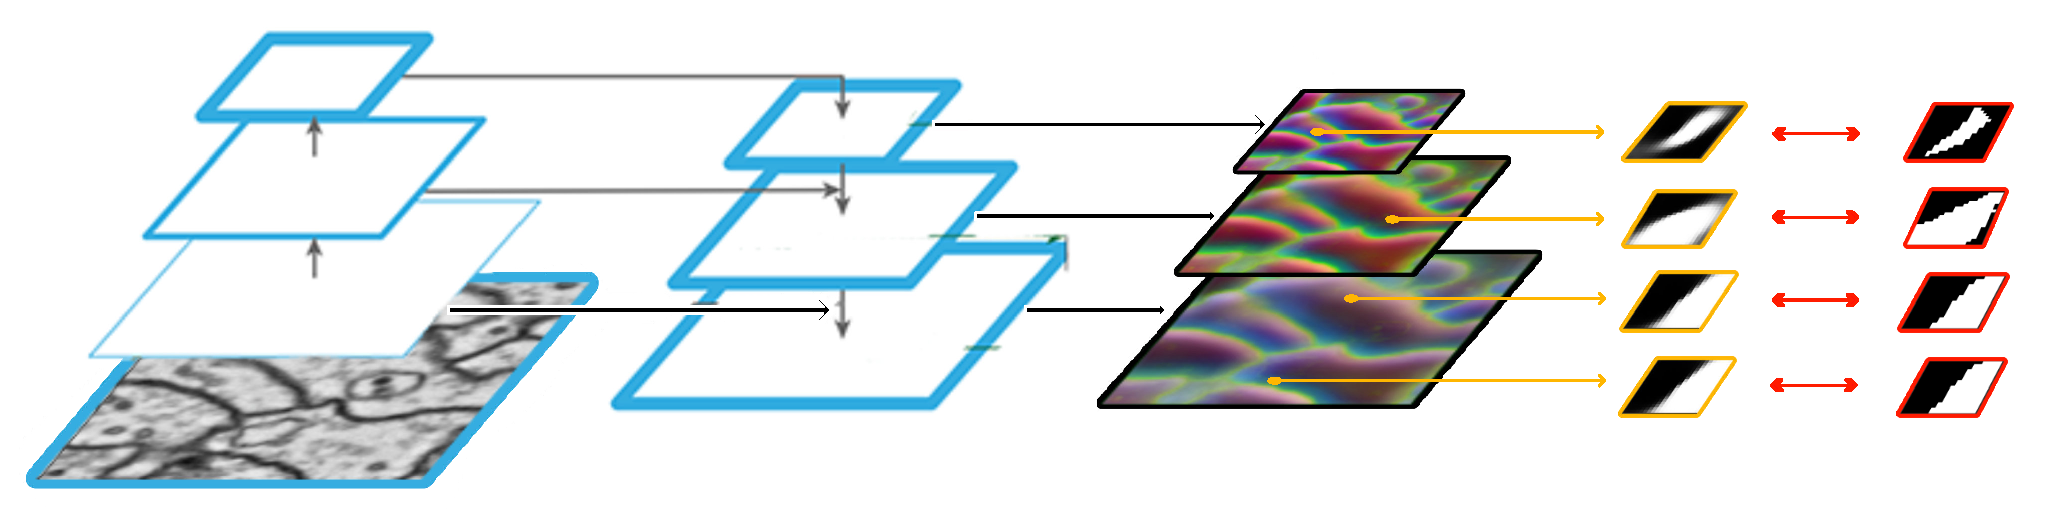
\includegraphics[width=\textwidth]{./figs/architecture.pdf} % 0.45
        \caption{Multi-scale patch prediction...}
    \label{fig:comparing_masks_affs}
\end{figure}


\textbf{Predicting pixel-pair affinities} --  
Instance-aware edge detection has experienced recent progress thanks to deep learning, both on natural images \cite{Gao_2019_ICCV,liu2018affinity,kirillov2017instancecut,xie2015holistically,kokkinos2015pushing} and biological data \cite{lee2017superhuman,schmidt2018cell,wolf2018mutex,bailoni2019generalized,meirovitch2016multi,ciresan2012deep}. Among these methods, the most recent ones also predict long-range affinities between pixels and not only direct-neighbor relationships.
Other related work \cite{funke2018large,turaga2009maximin} performs instead boundary detection via a structured learning approach.
In neuron segmentation, boundaries predicted by a CNN are converted to final instances with subsequent postprocessing and superpixel-merging.
Some methods use loopy graphs \cite{kaynig2015large,krasowski2015improving} or trees \cite{meirovitch2016multi,liu2016sshmt,liu2014modular,funke2015learning,uzunbas2016efficient,nunez2013machine,knowles2016rhoananet} to represent the region merging hierarchy. 
Others, define a graph with both positive and negative weights and formulates the problem in a combinatorial framework, known as \emph{multicut} or \emph{correlation clustering} problem \cite{kappes2011globally,chopra1991multiway,beier2017multicut}. 
In neuron segmentation and connectomics, exact solvers can tackle problems of considerable size \cite{andres2012globally}, but accurate approximations \cite{pape2017solving,beier2017multicut,beier2016efficient,yarkony2012fast,beier2014cut} and greedy agglomerative algorithms \cite{levinkov2017comparative,wolf2019mutex,bailoni2019generalized} have also been proposed.
% and persistence criteria \cite{lange2018partial,lange2018combinatorial} have been proposed for even larger graphs. 


